\chapter{Definition of Scenarios}
\label{anex:scenarios}

\section{Scenario 1: Emergencies - Lorca Earthquake (Spain)}
\subsection{Scenario description}
In May 11th of 2011, an Earthquake took place in Lorca, in the Region of Murcia (Spain) at 18:47 local time. It was a moderate magnitude $5.1$ in moment magnitude scale (M), preceded by a 4.5M foreshock at 17:05 local time. The seismic affected to other regions as Almería, Albacete, Granada, Jaén, Málaga, Alicante, Ciudad Real and Madrid. Several aftershocks occurred up to 3.9M in the following days. See (Instituto Geográfico Nacional) for more information.

Murcia is the most active seismic zone in Spain. Shortly after the second earthquake struck, the Spanish government, at the request of regional government of Murcia, activated the Military Emergencies Unit, a branch of the Spanish Armed Forces responsible for providing disaster relief. 

In these kind of natural disasters, emergencies units and humanitarian organizations demand accurate imagery before and after the disaster that has been proven to be very helpful to provide accurate \ac{GPS} navigation maps to reach affected areas, especially on developing and underdeveloped countries, as demonstrated in the 2010 Haiti earthquake or 2013 Haiyan Typhoon in Philippines (Hot).

\subsection{Response}

The Government needs the following service:
\begin{itemize}
\item The image of Lorca and surroundings before the first seismic activity is detected.
\item The image of Lorca and surroundings when the first seismic activity is detected.
\item The image of Lorca and affected regions in the day of the event is requested with urgency.
\item After this day:
\begin{itemize}
\item All the images daily acquired by the constellation are demanded during the first week, with urgency too, in order to manage emergency services and to assess the damages in the infrastructures. 
\item Until the first month after the earthquake, weekly images are requested without urgency. 
\item Then, monthly images also without urgency would be demanded until the
  first year after the event. 
\end{itemize}
\end{itemize}
The humanitarian organizations and volunteers may need:
\begin{itemize}
\item Images of Lorca before the earthquake, available through WMS and tiles.
\item Images of Lorca within the week after the earthquake, available through
  WMS and tiles.
\end{itemize}

\subsection{Data distribution}
The following data distribution mechanisms will be tested for this use case.
\begin{itemize}
\item \ac{FTP}: Scenes are distributed directly to the government via \ac{FTP} to be incorporated into the archives and used to their own criteria.
\item \ac{WMS}: To facilitate the analysis of the images to provide an adequate response to the event, a private \acl{WMS} will be provided. From the scenes of the affected region, composites images (mosaic) will be created and populated into the \ac{WMS} data store. The timestamp of the images will be incorporated to provide support to temporal requests; providing a TIME parameter with a time value in the WMS request does this. Having a WMS enables to have a rational distribution of images among the implicated organizations (firefighters, civil defense, army, etc.). The images can be requested only for needed times and regions by specifying time ranges and geographical area of interest. The WMS can be consumed from the GIS tools used by the emergency response organizations designated by the government.
\item Tiles: A public tiles service for the area of interest will be deployed. Humanitarian organizations and volunteers can create accurate maps of the affected area with these data. This service will have potentially high demand (thousands of volunteers accessing the service) in a very short period of time (during the crisis response). Tiles from imagery before and after the disaster will be published.
\end{itemize}

\subsection{Area of Interest} 
The \acl{AOI} is the Region of Murcia in Spain (see Figure~\ref{fig:region-murcia}). 

\begin{figure}[!h]
\begin{center}
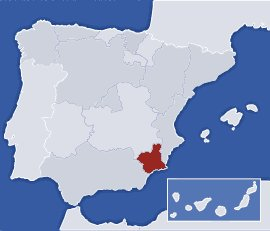
\includegraphics[width=0.7\textwidth]{detaildesign/region-murcia.jpg}
\caption{Region of Murcia (Spain) (image from \url{www.20minutos.es})}
\label{fig:region-murcia}
\end{center}
\end{figure}


\subsection{Users}
The main user of the service is the Spanish Government, and other organizations related to emergencies management. Other users could be volunteers and humanitarian organizations.
\subsection{Service Type}
The service type is a basic service that can eventually include a hosting service as well for the distribution of data to different emergency services and Estate Forces. Due to the urgency of the images, no added value would be required. 
\subsection{Processing Level}
The processing level will be low due to the urgent. In this scenario we do not contemplate added value services for damage assessment.
\subsection{Storage Level}
The storage level will be low.
\subsection{Communications Level}
The communication level is urgent.
\subsection{Demand Variability}
The demand is highly variable in this service.




\section{Scenario 2: Infrastructure monitoring. Affection in railway infrastructures by sand movement in desert areas (Spain)}
\subsection{Scenario description}
New high performance railway lines at ambient conditions characterized by the presence of wind, sand dunes, sand in the air and high temperatures, require innovative developments technology to minimize the impact of these phenomena on different infrastructure elements during the operation.
 

\begin{figure}[!h]
\begin{center}
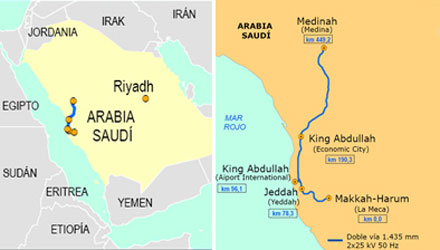
\includegraphics[width=0.7\textwidth]{detaildesign/arabia.png}
\caption[High Speed line Medina-La Meca in Saudi Arabia]{High Speed line Medina-La Meca in Saudi Arabia. Image from \url{https://www.thalesgroup.com/sites/default/files/asset/document/Gonzalo\%20Ferre.pdf}}
\label{fig:arabia}
\end{center}
\end{figure}

Remote sensing technologies can be applied to assess the risk of affection in the infrastructure and to minimize and prevent the impact: Sand movement and speed, risk maps, sand storms monitoring, floods monitoring, etc.

Satellite imagery can be combined with \ac{UAV}, with
higher resolution and flexible operation modes, to provide data to assist in the
deployment, operation and maintenance of these lines. 

\subsection{Response}
The solicited service is based on the following premises:
\begin{itemize}
\item Coverage during operation of the infrastructure.
\item Use of archive images to provide information about dunes movements and speed.
\item Monthly revisit time.
\item Urgent images only in case of storms and floods to inspect damages in the infrastructures.
\item The images require an analysis to identify risks zones, dune and sand
  speed fields, etc.
\end{itemize}

\subsection{Data distribution}
\begin{itemize}
\item \ac{WMS}: A Web Map Service will be deployed to distribute the scenes of the area of interest to the managers of the infrastructure. Imagery and derived products (risk maps, wind speed fields, etc.). 
\item Value added services (WFS, HTTP/REST, Tiles, etc.). Interactive value-added services may be provided to the managers in order to have monitoring tools. 
\end{itemize}
\subsection{Area of Interest}
Several areas of interest have been detected: The Medina-La Meca (Saudi Arabia) railway line currently in construction and the south of Spain (Andalucía) where testing technologies with sensors and \ac{UAV} are in development.
\subsection{Users}
\begin{itemize}
\item Private organizations, responsible of the construction and operation of the lines.
\item Public institutions responsible of the management of the railway
  infrastructures.
\end{itemize}

\subsection{Service Type}
The service type is advanced. It includes mosaics of the area of interest and combination with other sources of information.
\subsection{Processing Level}
The processing level is high
\subsection{Storage Level}
The storage level is high.
\subsection{Communications Level}
The communication level is not urgent.
\subsection{Demand Variability}
The demand is variable.

\section{Scenario 3: Land Management-South West of England}

\subsection{Scenario description}
There is a need to characterize landscape and crops in the South West of England, United Kingdom. Besides, the users demand a multitemporal product which allows analysing the land cover dynamics and detecting changes. For this task, multitemporal classification and regression techniques are used to provide products exploiting the high revisit time, high spatial resolution, high swath and large number of bands in the system (Sensyf).
\subsection{Response}
The primary focus of the service is Landscape Management linked to the use of the land for agricultural purposes versus conservation. 

The service is the following:
\begin{itemize}
\item Satellite images with a weekly frequency shall be offered, including the requested processing through a push type service.
\item Multitemporal Land Cover Classification and Change Detection Service are
  needed. Land cover and land cover change products will be generated from
  mosaics with the same temporal frequency, weekly, and service type, push.
\end{itemize}

\subsection{Data distribution}
\begin{itemize}
\item \ac{WFS} to provide direct access to the derived products: Land cover, etc.
\item Value-added services (REST/HTTP, WMS, Tiles) for the creation of web
  applications and interactive solutions. 
\end{itemize}

\subsection{Area of Interest} 
The Area of Interest is the South West of England, United Kingdom, see Figure~\ref{fig:england}.

 \begin{figure}[!h]
\begin{center}

\includegraphics[width=0.5\textwidth]{detaildesign/england.jpg}
\caption[South West of England]{South West of England (image from \url{http://www.holiday-home-dealers.co.uk/})}
\label{fig:england}
\end{center}
\end{figure}

\subsection{Users}
The user of this service is the European Landscape Convention.
\subsection{Service Type}
The service type is high added value (Push). Processing is required to offer the requested services: crops characterization, classification, irrigation planning, and change detection.
\subsection{Processing Level}
The processing level is medium.
\subsection{Storage Level}
The storage level is medium.
\subsection{Communications Level}
The communication level is not urgent since the changes in the crops are not immediate and the frequency of the images acquisition is higher than such changes. 
\subsection{Demand Variability}
The demand is variable. It depends on the season.

\section{Scenario 4: Precision Agriculture-Argentina}
\subsection{Scenario description}
Small farm operators, cooperatives, large agro-holdings, agricultural land
investment trusts, logistics and supply chain operators need homogeneous and
reliable means to manage their crops. Precision Agriculture provides support
services for irrigation, based on the use of \acl{EO} data, hydrological models and meteorological data. Using high resolution imagery, inadequate irrigation or practices can be identified quickly and other agricultural treatments can be more accurately assessed and optimized.

In Latin America the leading country is Argentina, where it was introduced in the middle 1990s with the support of the National Agricultural Technology Institute (Sensyf), (Astrium).
\subsection{Response}
The designed constellation will provide mosaics of Argentina in a daily basis, which shall be processed in order to offer several layers of precise information at the resolution of the satellite system to the users.
Some processing shall offer info about irrigation planning, improved management of fertilizer usage, meteorological data affecting crops and fruit maturity.
\subsection{Data distribution}
\begin{itemize}
\item \ac{WFS} to provide direct access to the derived products.
\item Value-added services (REST/HTTP, WMS, Tiles) for the creation of web
  applications and interactive solutions. 
\end{itemize}

\subsection{Area of Interest} 
The Area of Interest is Argentina, see Figure~\ref{fig:argentina}.

  \begin{figure}[!h]
\begin{center}
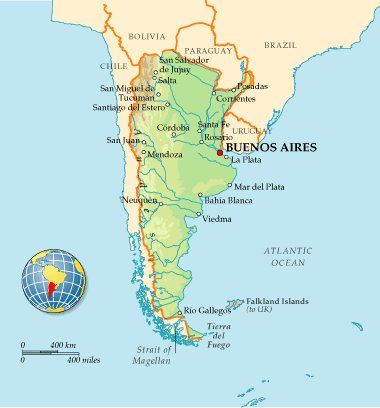
\includegraphics[width=0.7\textwidth]{detaildesign/argentina.jpg}
\caption[Map of Argentina]{Map of Argentina (from \url{http://www.dk.co.uk/static/cs/uk/11/worldfactfile/countries/ar.html})}
\label{fig:argentina}
\end{center}
\end{figure}

\subsection{Users}
The user is the National Agricultural Technology Institute.
\subsection{Service Type}
The service type is high added value (push/hosting) (subscription services for agriculture treatments, irrigation planning and general monitoring… Hosting could be employed for users that do not have where storage the data).
\subsection{Processing Level}
The processing level is high (several layers of post processing shall be offered to the users employing mosaics of the country, i.e. the National Agricultural Technology Institute).
\subsection{Storage Level}
The storage level is high. 
\subsection{Communications Level}
The communication level is not urgent.
\subsection{Demand Variability}
The demand variability is constant (depending on the season).

\section{Scenario 5: Basemaps-Worldwide}
\subsection{Scenario description}
Satellite operators, space agencies and mapping companies offer basemaps as part of their services and data product. Built from the satellite scenes, they provide seamless and cloud-free coverage of certain region surface (countries, continents and worldwide) with multiple zoom layers and high detail. They are distributed as data archives (\ac{FTP}, direct download) or through OGC Web Services (\ac{WMS}) and Tiles. These are some examples:
\begin{itemize}
\item NASA's Blue Marble: offers a year's worth of monthly composites at a spatial resolution of 500 meters. These monthly images reveal seasonal changes to the land surface: the green-up and dying-back of vegetation in temperate regions such as North America and Europe, dry and wet seasons in the tropics and advancing and retreating Northern Hemisphere snow cover. They are available for download as georreferenced raster files. 

\begin{figure}[!h]
\begin{center}
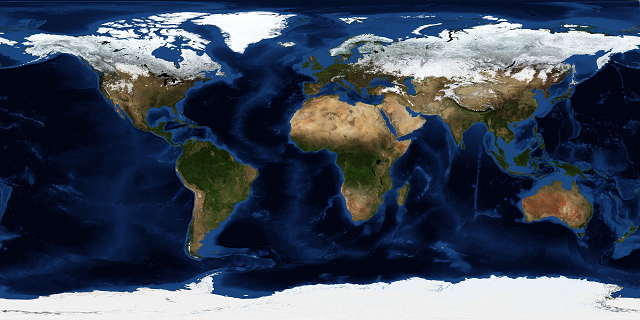
\includegraphics[width=0.9\textwidth]{detaildesign/basemap.png}
\caption{NASA's Blue Marble from December with topography and bathymetry (from \url{http://visibleearth.nasa.gov/view.php?id=73909}}
\label{fig:basemap}
\end{center}
\end{figure}
\item SPOTMaps: From Astrium, provides $2.5~m$, natural color, seamless
  ortho-mosaics derived from SPOT 5 data, providing nationwide and regional
  basemaps for a large part of the globe. They are currently available over more
  than 110 countries, and more than 94 million $km^2$. The coverage is growing
  and updated on a monthly basis.
\end{itemize}

\subsection{Response}
With the global daily coverage of the GEO-Cloud constellation of satellites, a monthly true-color basemap can be built with very high detail and coverage percentage (cloud-free). In tropical lowlands, cloud cover during the rainy season can be so extensive that obtaining a cloud-free view of every pixel of the area for a given month may not be possible.

Processing will consist of creating monthly mosaics from the daily coverage of the constellation, removing clouds and applying color adjustments to create true-color and visually attractive aerial basemaps.

Resolution of the basemaps will depend on the storage and processing capacity, it will be studied further during the implementation of the scenario.
\subsection{Data distribution}
Data will be delivered though cached \ac{WMS} and tiles.
\subsection{Area of Interest}
The area of interest is the whole world. Country or continent coverages can be represented. We will focus on Europe.
\subsection{Users}
\begin{itemize}
\item Governmental clients.
\item Infrastructure managers.
\item Third-party service providers.
\end{itemize}

\subsection{Service Type}
The service type is high added value (push/hosting), using on-line delivery mechanisms.
\subsection{Processing Level}
The processing level is high (creation of a monthly mosaic from a catalogue of
daily images, cloud removal or color adjustments)
\subsection{Storage Level}

The storage level is very high. It can be modulated with the maximum zoom level/resolution offered and the area of interest.
\subsection{Communications Level}
The communication level is not urgent.
\subsection{Demand Variability}
The demand variability is variable. See Table 14 for a summary of the service characteristics.